\section{Catmull-Clark}

\subsection{Allgemein}

Der Catmull-Clark Algorithmus wurde 1978 von Edwin Catmull und James Clark entwickelt.
Er ist eine Verallgemeinerung von bi-cubic uniform B-splines surfaces und arbeitet auf
Netzen mit beliebiger Topologie.
Das neu erzeugte Netz ist immer ein Vierecksnetz. Jedes n-Gon im Eingabenetz wird in n Quads
im Ausgabenetz umgewandelt.
Die Kontrollpunkte des Netzes werden durch Unterteilung approximiert.


\subsection{Unterteilungsregeln}

Um ein Kontrollnetz nach Catmull-Clark zu unterteilen sind vier Schritte notwendig.
\begin{enumerate}
	\item Füge für jedes Polygon einen neuen Punkt hinzu (face point).
	\item Füge für jede Kante einen neuen Punkt hinzu (edge point).
	\item Berechne für jeden alten Kontrollpunkt die neue Position (original point).
	\item Verbinde die Punkte (face point, edge point, original point), sodass diese ein
	neues verfeinerten Netz erzeugen (face split).
\end{enumerate}

\autoref{fig:sd_catmull_mask} zeigt die Masken, mit denen die jeweiligen Punkte für ein Viereck berechnet werden können.
Im folgenden wird der allgemeinere Fall für beliebige Polygone beschrieben.
\begin{figure}
\centering
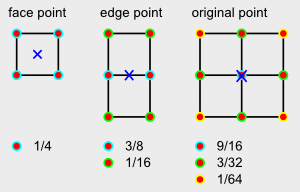
\includegraphics[width=0.5\textwidth]{content/media/sd_catmull_mask.png}
\caption{Catmull-Clark Maske für ein Viereck \cite{yoshihitoyagi.23.12.2015}}
\label{fig:sd_catmull_mask}
\end{figure}

\subsubsection*{Face Point}
Der Face Point berechnet sich als Mittelwert der Kontrollpunkte des Polygons.
Bei einem Viereck wie in \autoref{fig:sd_catmull_mask} hat somit jeder Kontrollpunkt
ein Gewicht von 1/4.

\subsubsection*{Edge Point}
Der Edge Point wird von den anliegenden Polygons beeinflusst.
Dieser errechnet sich aus dem Durchschnitt der zwei benachbarten Face Points und den
beiden Kontrollpunkten der Kante.

\subsubsection*{Original Point}
Jeder Original Point wird aktualisiert.
Die Berechnung wird folgendermaßen durchgeführt:\\
\(
new\_point=(Q/n) + (2R/n) + (S*(n-3)/n)\\
n:\ Valence\\
Q:\ Durchschnitt\ der\ umliegenden\ Face\ Points\\
R:\ Durchscnitt\ aller\ umliegenden\ Mittelpunkte\ der\ Ecken\ (!=\ edge\ point)\\
S:\ original\ Point
\)

\subsubsection*{Face Split}
Nun sind alle neuen Punkte berechnet.
Die Punkte müssen durch Kanten zu gültigen Quads zusammengesetz werden.
Ein Quad besteht aus den 4 Punkten:
\begin{itemize}
 \item Original Point
 \item Edge Point 1
 \item Face Point
 \item Edge Point 2
\end{itemize}
Für jedes Polygon mit n Ecken entstehen n Quads.
\cite{rosettacode.23.12.2015}
\cite{rorydriscoll.23.12.2015}
\cite{yoshihitoyagi.23.12.2015}



\subsection{Sonderfälle}


